\documentclass[../main.tex]{subfiles}

\begin{document}

\begin{figure}
    \centering
    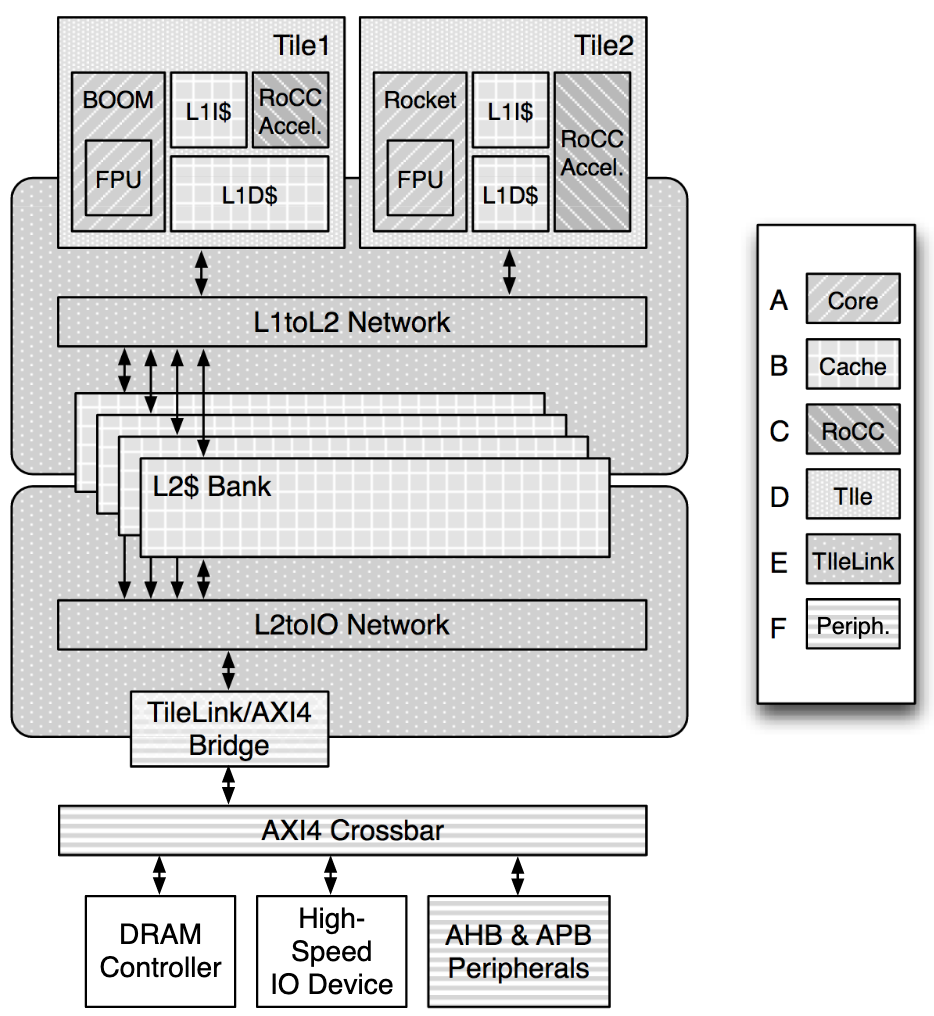
\includegraphics[scale=.5]{pngs/RocketChipGeneratorLayout.png}
    \caption{Rocket Chkp Pipeline\cite{Asanović:EECS-2016-17}}
    \label{fig:RocketCipGen}
\end{figure}
The Rocket Core was generated by using the Rocket Chip Generator. The Rocket Chip Generator was developed by UC. Berkeley and is maintained by the CHIPS Alliance. Figure \ref{fig:RocketCipGen} shoe a high level overview of a default Rocket Chip. 

Starting form top to bottom: The Generator can be used to create N Number of Tiles. Tiles are the most basic building block in the system. It contains a processor, L1 instruction cache, L1 data cache and ROCC Accelerator. The ROCC Accelerator can be any custom function that is required for a specific application. One of noteworthy accelerator is the Hwacha Vector-Fetch Architecture\cite{HwachaPaper}. Each Tile is connected together by the L1toL2 Network. Next, is the L2 Cache banks. The L2 Cache banks are connected to L2toIo Network. This network is entry point for the Rocket Core in to a global system.
\subsection{RISC-V Processor}
The default RSIC-V Processor is called the Rocket Core. The Rocket Core is a single fetch, single issue, in-order scalar processor. The RISCV ISA allows for 
\end{document}